\subsection{Homotopy-based Path-Planning}

\subsubsection{Algorithm}

\begin{frame}{Homotopy in Path-Planning}{Homotopy-based Path-Planning}
	
\begin{columns}
\column{.45\textwidth}
\begin{figure}
	\centering
	\begin{subfigure}
		\centering
		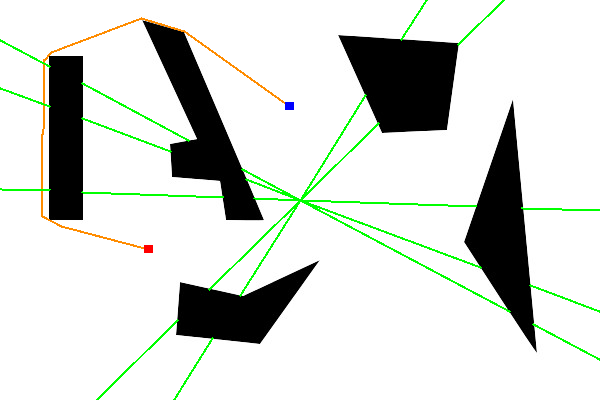
\includegraphics[width=.47\textwidth]{figure/all_homotopy_classes/s1.png}
	\end{subfigure}  
	\begin{subfigure}
		\centering
		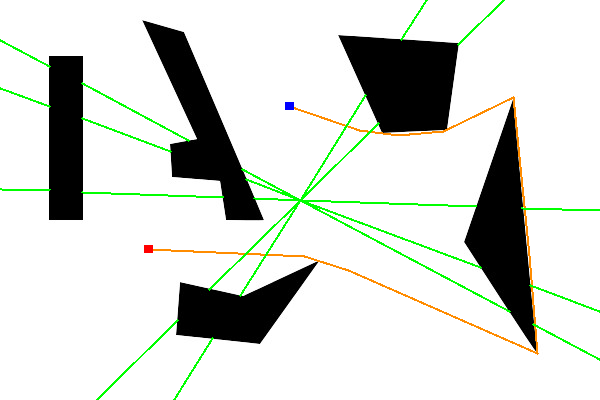
\includegraphics[width=.47\textwidth]{figure/all_homotopy_classes/s2.png}
	\end{subfigure}
	\\
	\begin{subfigure}
		\centering
		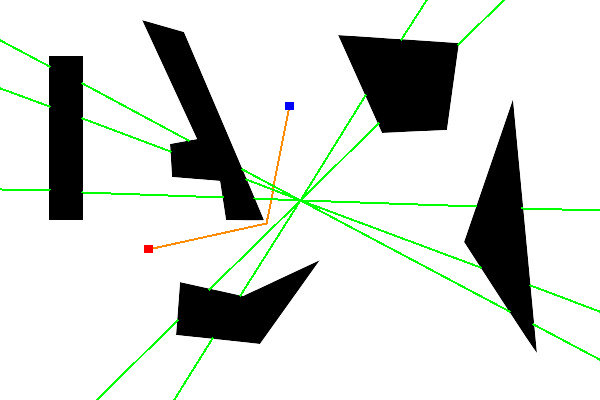
\includegraphics[width=.47\textwidth]{figure/all_homotopy_classes/s3.png}
	\end{subfigure}  
	\begin{subfigure}
		\centering
		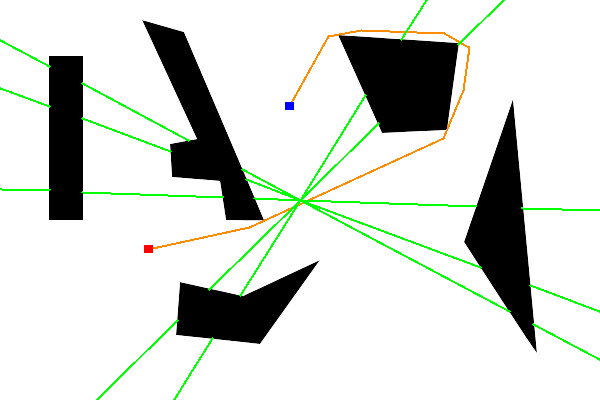
\includegraphics[width=.47\textwidth]{figure/all_homotopy_classes/s4.png}
	\end{subfigure}
	\\
	\begin{subfigure}
		\centering
		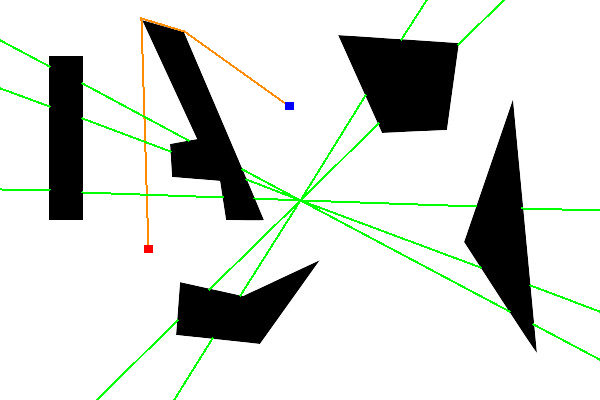
\includegraphics[width=.47\textwidth]{figure/all_homotopy_classes/s5.png}
	\end{subfigure}	 
	\begin{subfigure}
		\centering
		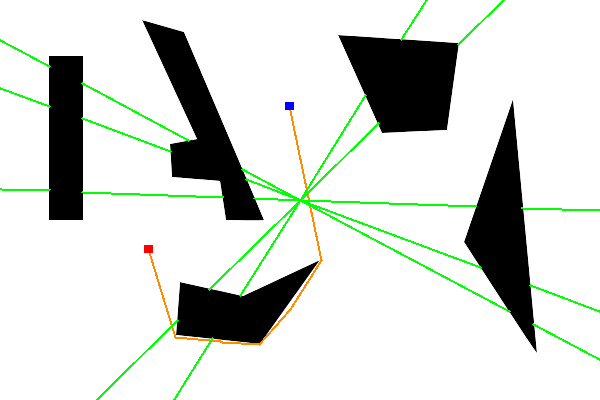
\includegraphics[width=.47\textwidth]{figure/all_homotopy_classes/s6.png}
	\end{subfigure}	 
\end{figure}
\column{.52\textwidth}
\begin{block}{Hard Constraint}
\begin{itemize}
\item Specific homotopy class
\item Via-regions / Forbidden regions
\end{itemize}
\end{block}
\begin{block}{Soft Constraint}
\begin{itemize}
\item Homotopy preference
\end{itemize}
\end{block}
\end{columns}
	
\end{frame}

\begin{frame}{Homotopy-based Optimal Path-Planning}{Homotopy-based Path-Planning}
	
\begin{columns}
\column{.45\textwidth}
\begin{figure}
	\centering
	\begin{subfigure}
		\centering
		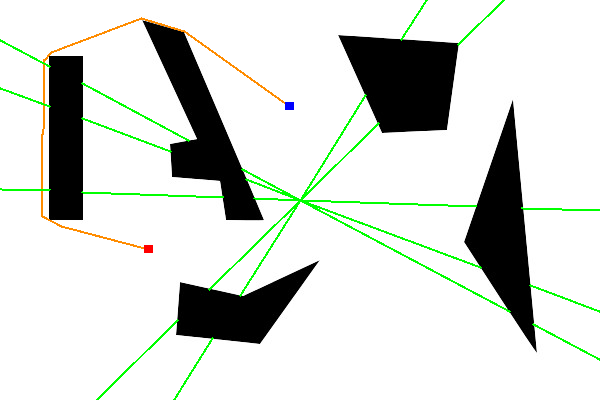
\includegraphics[width=.47\textwidth]{figure/all_homotopy_classes/s1.png}
	\end{subfigure}  
	\begin{subfigure}
		\centering
		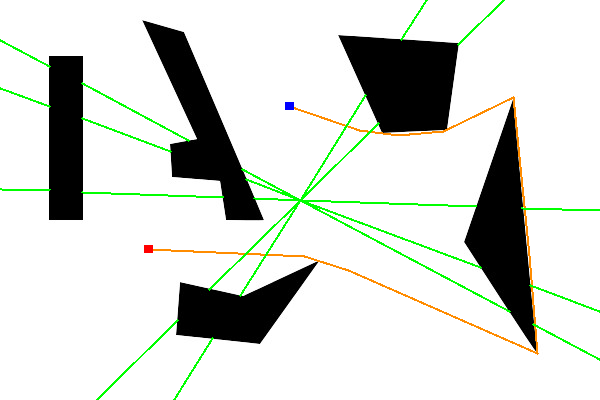
\includegraphics[width=.47\textwidth]{figure/all_homotopy_classes/s2.png}
	\end{subfigure}
	\\
	\begin{subfigure}
		\centering
		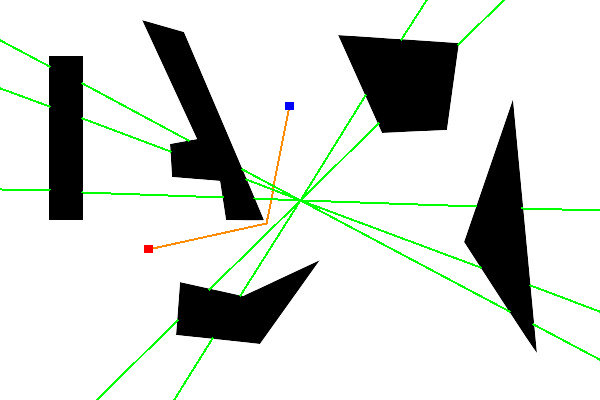
\includegraphics[width=.47\textwidth]{figure/all_homotopy_classes/s3.png}
	\end{subfigure}  
	\begin{subfigure}
		\centering
		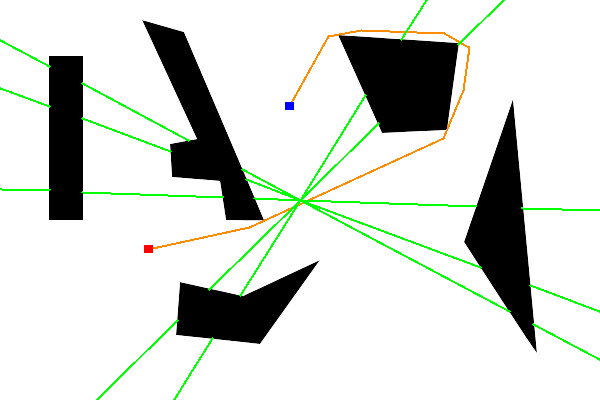
\includegraphics[width=.47\textwidth]{figure/all_homotopy_classes/s4.png}
	\end{subfigure}
	\\
	\begin{subfigure}
		\centering
		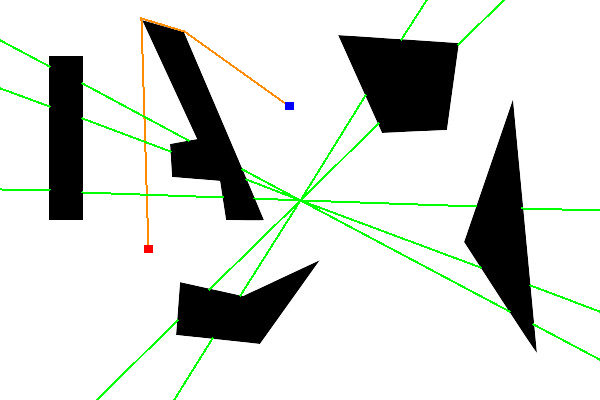
\includegraphics[width=.47\textwidth]{figure/all_homotopy_classes/s5.png}
	\end{subfigure}	 
	\begin{subfigure}
		\centering
		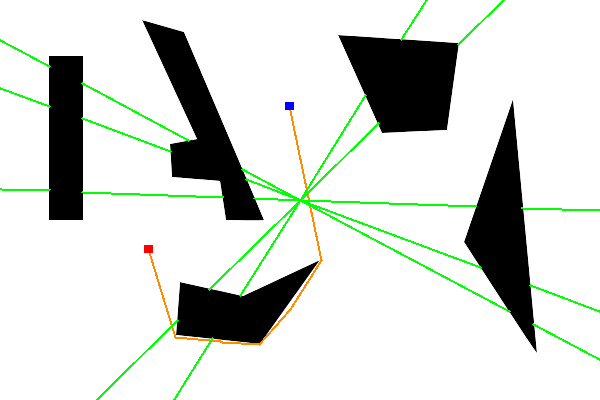
\includegraphics[width=.47\textwidth]{figure/all_homotopy_classes/s6.png}
	\end{subfigure}	 
\end{figure}
\column{.52\textwidth}
\begin{block}{Optimal Paths of Homotopy Classes}
\begin{itemize}
\item $ \bm{H} ( x_{init}, x_{goal} ) $ - the set of homotopy classes defined by $ x_{init} $ and $ x_{goal} $
\item $ H = { h_1 , \cdots , h_N } \subseteq \bm{H} $
\item $ \forall h_i \in H, \sigma^{*}_{h_i} = \arg \min_{\sigma \in X_{\it free} \land h(\sigma) = h_i } \mbox{\sc Cost}  (\sigma) $
\end{itemize}
\end{block}
\end{columns}
	
\end{frame}

\begin{frame}{Homotopy-based Optimal Path-Planning}{Homotopy-based Path-Planning}

{\bf Solution}

\begin{block}{}
Convert a path into a string representation
\end{block}
\begin{block}{}
Determine the homotopic equivalence by string representation
\end{block}
\begin{block}{}
Find the optimal paths by string representation
\end{block}

\end{frame}

\begin{frame}{Generate String Representation}{Homotopy-based Path-Planning}

\begin{columns}

\column{.4\textwidth}
\begin{figure}
	\centering
	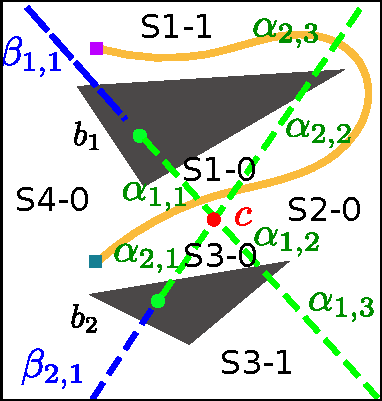
\includegraphics[width=\linewidth]{figure/obs_map}
\end{figure}
\column{.57\textwidth}
\begin{itemize}
\item A ray structure decomposes the map
\item Reference frames with ID
\item How a path sequentially crosses reference frames generates a string of IDs
\end{itemize}
\end{columns}

\end{frame}

\begin{frame}{Homotopy Equivalence}{Homotopy-based Path-Planning}

\begin{columns}

\column{.33\textwidth}
\begin{figure}
	\centering
	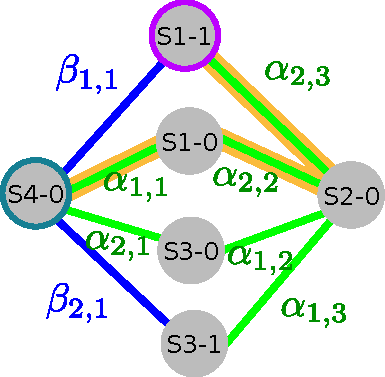
\includegraphics[width=\linewidth]{figure/obs_topology}
\end{figure}
\column{.05\textwidth}
\begin{figure}
	\centering
	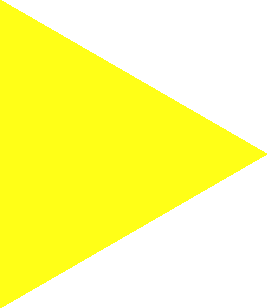
\includegraphics[width=\linewidth]{figure/arrow2}
\end{figure}
\column{.3\textwidth}
\begin{figure}
	\centering
	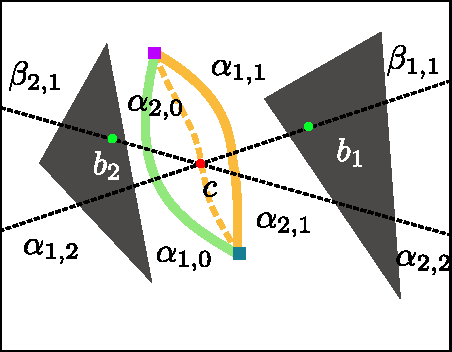
\includegraphics[width=\linewidth]{figure/equivalence1}
\end{figure}
\begin{figure}
	\centering
	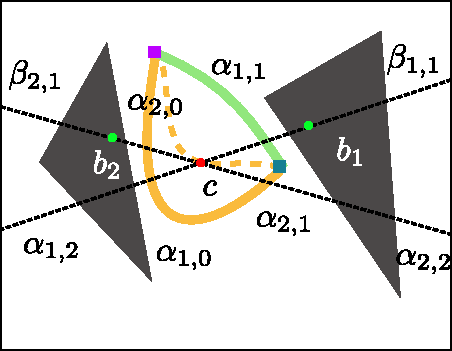
\includegraphics[width=\linewidth]{figure/equivalence2}
\end{figure}
\column{.05\textwidth}
\begin{figure}
	\centering
	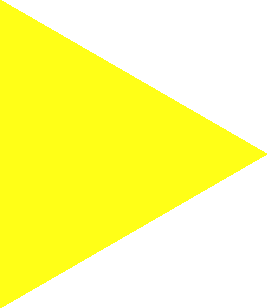
\includegraphics[width=\linewidth]{figure/arrow2}
\end{figure}
\column{.18\textwidth}
\begin{figure}
	\centering
	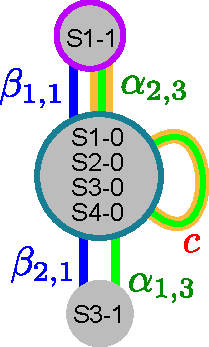
\includegraphics[width=\linewidth]{figure/obs_topology2}
\end{figure}
\end{columns}

\end{frame}

\begin{frame}{Homotopy-Aware Optimal Search}{Homotopy-based Path-Planning}

\begin{columns}

\column{.33\textwidth}
\begin{block}{RRT*}
\begin{figure}
	\centering
	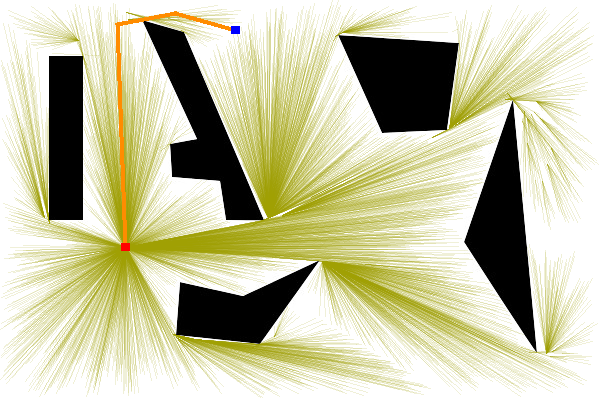
\includegraphics[width=\linewidth]{figure/single_tree}
\end{figure}
\end{block}
\column{.33\textwidth}
\begin{block}{Bi-RRT*}
\begin{figure}
	\centering
	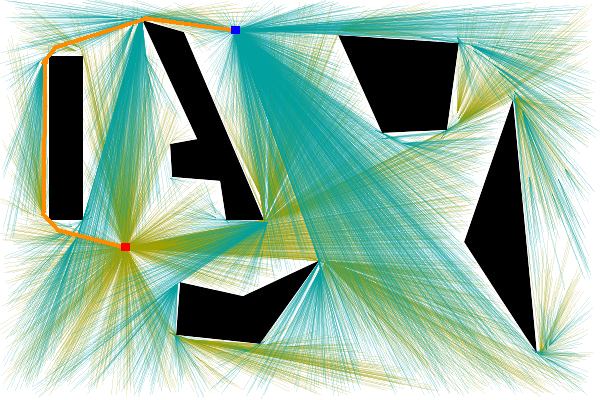
\includegraphics[width=\linewidth]{figure/bi_tree}
\end{figure}
\end{block}
\column{.33\textwidth}
\begin{block}{RRG*}
A graph structure
\begin{figure}
	\centering
	
\includegraphics[width=.5\linewidth]{figure/question_mark}
\end{figure}
\end{block}
\end{columns}

\end{frame}

\subsubsection{Validation}

\begin{frame}{Validation - Theoretical Analysis}{Homotopy-based Path-Planning}
	
{\bf The Mapping between Homotopy Classes and String Blocks}

\begin{figure}
	\centering
	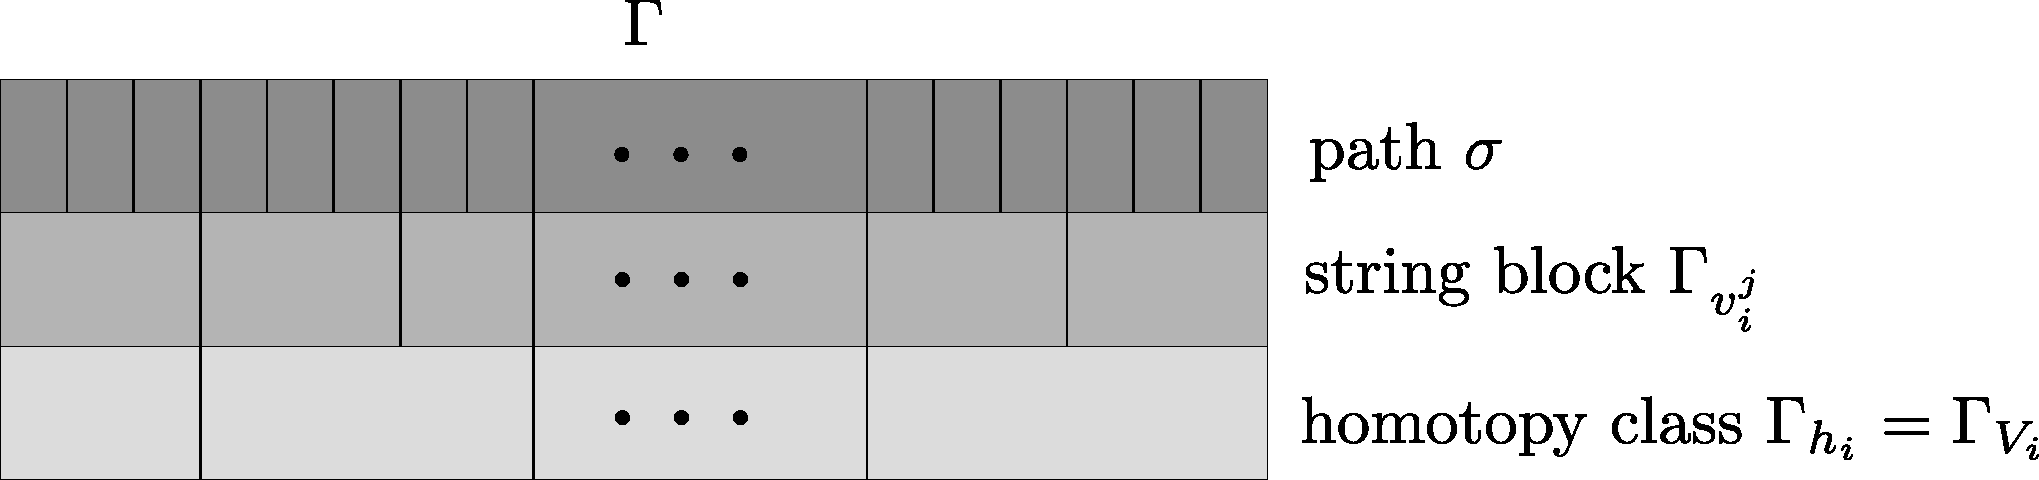
\includegraphics[width=.7\linewidth]{figure/decomp_hierarchy}
\end{figure}

\begin{thm}
${\rm REPTrim}(\bm{M}^h(\sigma_i)) =  {\rm REPTrim}(\bm{M}^h(\sigma_j )) $\footnotemark
 iff $\sigma_i \simeq \sigma_j$.
\end{thm}	
	
\footnotetext[1]{ $ \bm{M}^h() $ is a DFA that converts a path into a string.}	
	
\end{frame}

\begin{frame}{Validation - Theoretical Analysis}{Homotopy-based Path-Planning}

\begin{thm}
The solutions of the proposed algorithm can find the optimal paths of all simple homotopy classes\footnotemark.
\end{thm}

\begin{itemize}
\item All the simple homotopy classes would be explored.
\item The solutions of all the simple homotopy classes converge to optimal.
\end{itemize}


\footnotetext[1]{{\bf Simple homotopy class} is defined as a homotopy class of paths that do not form complete loops around obstacles.}

\end{frame}

\begin{frame}{Validation - Simulation}{Homotopy-based Path-Planning}

\begin{columns}[t]

\column{0.32\textwidth}
\begin{block}{Optimal Search}
\begin{itemize}
\item RRT*
\item Bi-RRT*
\item RRG 
\end{itemize}
\end{block}

\column{0.32\textwidth}
\begin{block}{Environment}
\begin{itemize}
\item Simple obstacles
\item Complex obstacles
\end{itemize}
\end{block}

\column{0.32\textwidth}
\begin{block}{Constraint}
\begin{itemize}
\item Single Homotopy Class
\item Multiple Homotopy Classes
\end{itemize}
\end{block}

\end{columns}

\end{frame}